%\documentclass[a4paper,10pt]{article}
\documentclass[conference]{format/IEEEtran}
%\usepackage[utf8x]{inputenc}
\usepackage[utf8]{inputenc}
\usepackage{graphicx}
\usepackage{url}


%opening
\title{Automatic Detection of Bad Programming Habits in Scratch: A Preliminary Study}
%\author{Jesús Moreno, Gregorio Robles}

\author{\IEEEauthorblockN{Jesús Moreno}
\IEEEauthorblockA{Programamos.es \& Instituto Nacional de \\ Tecnologías Educativas y de Formación del Profesorado\\
Madrid, Spain\\
jesus.moreno@programamos.es}
\and
\IEEEauthorblockN{Gregorio Robles}
\IEEEauthorblockA{GSyC/LibreSoft\\Universidad Rey Juan Carlos\\
Madrid, Spain\\
grex@gsyc.urjc.es}}


\begin{document}

\maketitle

\begin{abstract}
%This paper describes a method for automatic detection of two bad programming habits that students learning to program with Scratch incur, such as the repetition of code and object naming, and raises ideas to try to avoid such situations. FIXME: some methodology, results and conclusions should be included in the abstract.
Using the Scratch environment as a tool to teach programming skills or develop computational thinking is increasingly common in all levels of education, well-documented case studies from primary school to university can be found.

However, there are reports that indicate that students learning to program in this environment show certain habits that are contrary to the basic programming recommendations. In our work as instructors with high school students, we have detected these and other bad practices, such as the repetition of code and object naming, on a regular basis. This paper focuses on verifying whether these issues can generally be found in the Scratch community, by analyzing a large number of projects available on the Scractch community website.

To test this hypothesis, we downloaded 100 projects and analyzed them with two plug-ins we developed to automatically detect these bad practices. The plug-ins extend the functionality of the Hairball tool, a static code analyzer for Scratch projects. 

The results obtained show that, in general, projects in the repository also incur in the investigated malpractices. Along with suggestions for future work, some ideas that might assist to address such situations are proposed in the conclusions of the paper.
\end{abstract}

\section{Introduction}

Scratch~\cite{resnick2009scratch}  is a programming environment including a visual programming language designed for children over 6 years old, a development environment and a website where the community can host their projects, run, study and reuse other programs, and share ideas or suggestions with other programmers. Although there are several similar visual programming languages, Scratch is undoubtedly the most successful one with more than three million registered users in its website and more than five million shared projects in its repository\footnote{See \url{http://scratch.mit.edu/statistics/}}.

Scratch is being used both in extracurricular activities~\cite{kafai2010entering} or summer camps~\cite{adams2010scratching}, as in elementary schools~\cite{wilson2012evaluation}, high schools~\cite{meerbaum2013learning} and even universities worldwide~\cite{malan2007scratch}. Its capacity to bring computer programming to children and teenagers with the aim of fostering computational thinking abilities and to promote ICT studies, and its success to teach both basic and advanced programming concepts (concepts such as user interaction, conditional statements, communication and synchronization, logical expressions and data representation are taught) has been well documented~\cite{maloney2008programming, franklin2013assessment, wolz2009starting}.

However, it is also possible to find studies that have detected some bad programming habits in students learning to program in this environment~\cite{meerbaum2011habits}. In this line, in our work as instructors we have also found some bad habits despite having insisted our students to avoid them. As these habits are contrary to the basic programming recommendations, our study tries to find out if they are also common in the projects shared in the Scratch repository. 

%FIXME: the goal of this paper is to... 
The goal of this paper, therefore, is to determine whether these bad habits are common practices in the Scratch community in an automatic manner and propose some ideas to try to avoid such situations. In order to assist evaluators to detect these malpractices we have developed two plug-ins that automate the detection of the bad programming practices by extending the functionality of Hairball, a static code analyzer of Scratch projects.

The structure of this paper is as follows: In section~\ref{sec:background} a brief overview of Scratch is presented, including some research studies that have investigated learning in this environment and other studies that automate the evaluation of learning. In section~\ref{sec:methodology} our work methodology is briefly described. Section~\ref{sec:findings} presents the results we have obtained from applying our methodology on a small sample of Scratch projects. Finally, Section~\ref{sec:conclusions} contains the conclusions of our study and some ideas and suggestions for future work are discussed.

\section{Background}
\label{sec:background}

Scratch is a visual programming environment, developed by the Lifelong Kindergarten group at the MIT Media Laboratory, that allows to program interactive projects using a drag-and-drop approach with different pieces or \textit {Lego} style blocks~\cite{resnick2009scratch}. Scratch was designed with the main goal of encouraging young people to program, and most of its users are novice learners with no prior programming experience~\cite{maloney2010scratch}. The environment is designed to encourage users to manipulate and modify various media types, so that children and teenagers can create projects that they find interesting and attractive, such as animated stories, games or interactive presentations~\cite{maloney2008programming}.

Scratch also offers a website where the projects programmed by the community are published. The code of programs hosted there can be run, and following the community idea of the free software movement it can be studied and analyzed. So, it is possible to make suggestions and to reuse the code, and there are lots of valuable resources available for anyone willing to start to program. This approach offers as well the opportunity to learn social skills related to programming and beyond, such as sharing and contributing to the community~\cite{scaffidi2012skill}.

% repe
%There are many papers showing that Scratch works as a tool for learning to program~\cite{maloney2008programming, franklin2013assessment, scaffidi2012skill, malan2007scratch}, and there are success stories at different educational levels, environments and disciplines showing that students learn concepts such as user interaction, conditional statements, communication and synchronization, logical expressions and data representation.

Despite the positive impact of Scratch, Meerbaum-Salant, Armoni and Ben-Ari~\cite{meerbaum2011habits} prove that students learning to program in this environment show some bad habits that are contrary to recommended programming practices. In particular, they show a tendency to excessive decomposition and a bottom-up development process, starting with individual blocks of Scratch.

Aiming to simplify the process of evaluating computational thinking and help evaluators with an automatic tool, Hairball was created~\cite{boe2013hairball}. Hairball is a static analyzer of Scratch projects inspired by Lint\footnote{\url{http://www.unix.com/man-page/FreeBSD/1/lint}} that tries to detect programming errors in Scratch projects, such as not initializing the value of a variable or the state of a character, sending messages that are not received by any program, including code that is never run, among others.

\section{Methodology}
\label{sec:methodology}

In our work as instructors with high school students, we found that, despite our constant insistence and warnings, many students show on a regular basis two bad habits that have to do with object naming and code repetition:

\begin{enumerate}

  \item Students do not change the names of the characters, which are automatically named by the environment as \textit{SpriteX} where X is an incremental number. When the amount of characters in a project is large, it becomes very hard to know what object relates to a given statement, contributing to poor code readability, slowing the project programming, and complicating debugging to fix bugs.

  \item Students repeat code in the same project, sometimes even in the same character programs. Thus, abstraction and modularization, two key components of the development of computational thinking~\cite{wing2008computational}, are not trained. And the \emph{code base} becomes more complicated to maintain and update in the future.

\end{enumerate}

In order to detect these two behaviors in Scratch projects automatically, we have developed following plug-ins for the Hairball environment~\cite{boe2013hairball}, which in turn make use of \textit{kurt}\footnote{\url{https://github.com/blob8108/kurt}}, a library implemented in Python. The developed plug-ins are:

\begin{enumerate}

  \item \textit{convention.SpriteNaming}\footnote{\url{https://github.com/jemole/hairball/blob/master/hairball/plugins/convention.py}} analyzes a Scratch project to check if the names of its characters begin with the string \textit{Sprite}, indicative for the user not having changed the default name.

As an example to illustrate the drawbacks associated with this bad programming behavior, Fig.~\ref{fig:SpriteNaming} shows a script that is difficult to read because the complete character area has to be explored to find what character refers to a particular block. This makes the program difficult to debug should errors arise, making it hard to improve the code and slowing down the programming tasks. 

\begin{figure}
  \centering
    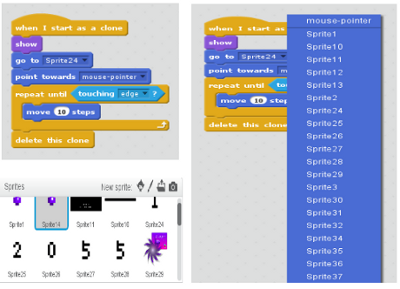
\includegraphics[width=9cm]{img/SpriteNaming.png}
  \caption{Sprites with default names}
  \label{fig:SpriteNaming}
\end{figure}

  \item \textit{duplicate.DuplicateScripts}\footnote{\url{https://github.com/jemole/hairball/blob/master/hairball/plugins/duplicate.py}} analyzes a Scratch project to try to locate repeated complete programs within a project. In order to do so, the plug-in runs each script of the project and gets the \textit{tokens} of the different blocks of the programs, so that two blocks that only differ in the values they receive are considered to be equal. A minimum length of five blocks is applied for programs to be considered duplicate rather than coincidentally similar.
  
  To illustrate the operation of this plug-in, Fig.~\ref{fig:CodeRepetition1} shows two scripts containing the same blocks with the only difference of the values received by parameter.


\begin{figure}
  \centering
    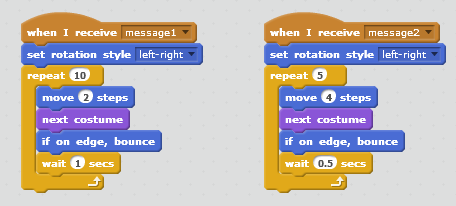
\includegraphics[width=9cm]{img/CodeRepetition1.png}
  \caption{Two scripts repeating code}
  \label{fig:CodeRepetition1}
\end{figure}


The Scratch scripts are analyzed by the plug-in and translated into \textit{tokens}. The analysis would result in considering them equal, as their code would be translated in both cases into the following sequence of \textit{tokens}:
\begin{verbatim}
 'set rotation style %s'
 'repeat %s%s'
 'move %s steps'
 'next costume'
 'if on edge, bounce'
 'wait %s secs'
\end{verbatim}

Hence, the correct way to implement this functionality would have been as shown in Fig.~\ref{fig:CodeRepetition2}, defining a new set of blocks that receives several values per parameter, and then reusing the block created in both programs. This solution would facilitate future maintenance, updating and debugging.

\begin{figure}
  \centering
    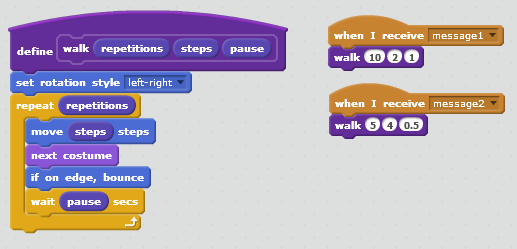
\includegraphics[width=9cm]{img/CodeRepetition2.png}
  \caption{Definition of blocks to avoid code repetition.}
  \label{fig:CodeRepetition2}
\end{figure}

\end{enumerate}


In order to test the functionality of the developed plug-ins and to verify whether these behaviors are common in projects found in the Scratch repository, we proceeded to randomly download 100 projects from the repository. As the possibility for users to define their own blocks, using \textit{def\_block} feature, is only available since the release of Scratch 2.0, we selected and downloaded projects created for this version. A replication package of the projects under study, and the specific version of the plug-ins used in it can be obtained publicly\footnote{FIXME: URL \url{http://gsyc.urjc.es/~grex/repro/2014-fie-scratch}}.


\section{Findings}
\label{sec:findings}

The results obtained after analyzing the 100 projects confirm that observations made with our students can also be generally found in the community projects, as shown in table \ref{table:results}.

Regarding the lack of habit of renaming the characters and not using the default name assigned by the environment, 79\% of the analyzed projects contained at least one non-renamed \textit{SpriteX} character.

As for the repetition code, 62\% of the analyzed projects contained at least one repeated program. In fact, only 17\% of the analyzed projects made use of block \textit{def\_block} to define its own blocks that can be reused in other parts of the project. 

FIXME: here comes the table with some more results. Important: to note how the distribution (talk about mean and median).

\begin{table}
\begin{center}
  \begin{tabular}{ | p{2.5cm} | p{1cm} | p{1.2cm} | p{1cm} |}
   \hline
     & Default names & Duplicated scripts & Defined blocks \\ \hline\hline
    Projects incurring in & 79 & 62 & 17 \\ \hline
    Mean & 5.94 & 7.23 & 1.11 \\ \hline
    Median & 3 & 2 & 0 \\ \hline
    Maximum & 67 & 71 & 25 \\
    \hline    
  \end{tabular}
\end{center}
\caption{Table of results}
\label{table:results}
\end{table}








\section{Conclusions and further research}
\label{sec:conclusions}

%FIXME: In this paper... short summary of what we have done and why

This paper shows the preliminary results of a study regarding two bad programming habits we have detected in our work as instructors with high school students learning to program with Scratch. In order to check if these bad habits, which have to do with object naming and code repetition, are also commonly found in the projects shared in the community repository, we downloaded 100 projects and analyzed them with two plug-ins we developed for Hairball, detecting that most of the inspected projects, 79\% and 62\%  respectively, fall into these issues.

Regarding object naming, it is worth to note that Scratch users name the variables used in their projects correctly, i.e., semantically meaningful. In our opinion the reason to explain this paradox is because it is mandatory to assign a name to a variable the moment it is created, as the environment does not name it by default. However, when creating a new character a  \textit{SpriteX} name is assigned automatically. In our views, a change of this feature of the environment, forcing users to name new objects, might eliminate this bad practice.

Regarding code repetition and the low usage Scratch users make of the possibility of creating their own blocks (the equivalent of defining methods or procedures in other languages), works as the one performed by Seiter and Foreman~\cite {seiter2013modeling}, in which they show that abstraction and modularization capacities are concepts that seem to be developed from a certain age, may explain the low rates of use of this functionality, since a significant part of the Scratch community consists of children under 10 years\footnote{\url{http://scratch.mit.edu/statistics/#age}}. Future studies should further investigate how to continue advancing in the definition of an appropriate framework for different ages, as well as to check whether users learning online and those who do it in a regulated environment show different use rates of this functionality.

%In the near future, we plan to... FIXME... talk about next steps: i) more analysis, ii) more projects, iii) web-based tool that provides learning-oriented feedback in an automatic way.

In the near future we plan to extend the scope of our study developing new plug-ins to automate the detection of other issues, such as the degree of development of computational thinking demonstrated in a project, and by analyzing a much larger number of projects to achieve more accurate conclusions. In this sense, the release of a research dataset with the first five years of data from the Scratch repository\footnote{\url{https://sites.google.com/site/scratchdatameeting/}} will be certainly a great help to our work. Finally, we are in the process of developing a website that will allow students to receive immediate feedback for their programs with warnings of potential errors and tips to improve their code.

\section*{Acknowledgments}

The work of Gregorio Robles has
been funded in part by the Spanish Government under project 
SobreSale (TIN2011-28110) and under project ``eMadrid - Investigación y Desarrollo de tecnologías para el e-learning en la Comunidad de Madrid'' (S2009/TIC-1650) funded by the Region of Madrid.

\bibliographystyle{abbrv}
\bibliography{scratch}
\end{document}
